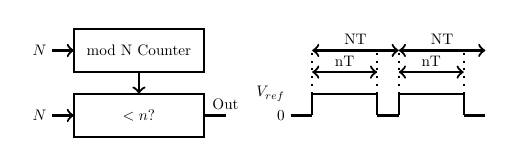
\begin{tikzpicture}[thick, transform shape, scale=0.55]
	\draw node at (0.5,0) [anchor=east] {$N$};
	\draw [->] (0.5,0) -- (1,0);
	\draw (1,0.5) rectangle (4,-0.5);
	\draw node at (2.5,0) {mod N Counter};
	
	\draw [->] (2.5,-0.5) -- (2.5,-1);
	
	\draw node at (0.5,-1.5) [anchor=east] {$N$};
	\draw [->] (0.5,-1.5) -- (1,-1.5);
	\draw (1,-1) rectangle (4,-2);
	\draw node at (2.5,-1.5) {$<n?$};
	
	\draw (4,-1.5) -- (4.5,-1.5) node [anchor=south] {Out};
	
	%PWM Signal:
	\node at (6,-1) [anchor=east] {$V_{ref}$};
	\node at (6,-1.5) [anchor=east] {$0$};
	
	\foreach \x in {6.5,8,8.5,10}
	{
		\draw (\x,-1) -- (\x,-1.5);
		\draw [dotted] (\x,-1) -- (\x,0);
	}
	\foreach \x in {6,8,10}
		\draw (\x,-1.5) -- (\x+0.5,-1.5);
	\foreach \x in {6.5,8.5}
		\draw (\x,-1) -- (\x+1.5,-1);
	
	\foreach \x in {6.5,8.5}
	{
		\draw [<->] (\x,0) -- (\x+2,0);
		\node at (\x+1,0) [anchor=south] {NT};
	}
	\foreach \x in {6.5,8.5}
	{
		\draw [<->] (\x,-0.5) -- (\x+1.5,-0.5);
		\node at (\x+0.75,-0.5) [anchor=south] {nT};
	}

\end{tikzpicture}